\chapter{Methodology}

\section{System Block Diagram}

\begin{figure}[ht]
\centering
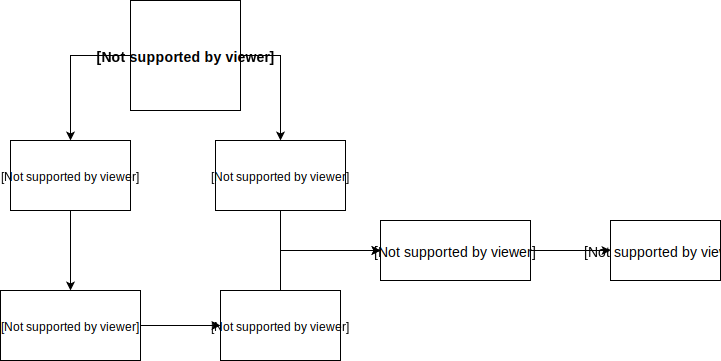
\includegraphics[width=1\linewidth]{mainmatter/3-Methodology/images/block.png}
\caption{System Block Diagram}
\label{fig:system}
\end{figure}

{The figure }~\ref{fig:system}
{
shows the various components used to form the prediction system. The idea is basic in that protein interaction depends on the structural and chemical properties. The structural components are fulfilled and
}

\section{Dataset}

\subsection{KEGG}
It is a community-driven database which holds large-scale molecular datasets generated by genome sequencing and high-throughput experimental techniuqe.\cite{Kanehisa2000} We use KEGG DRUG dataset for finding the interaction set between DRUG and PROTEIN. The interaction score is based on:

\begin{flushright}
\begin{equation}
  KIBA = \begin{cases}
    K_i . {adj} & \quad {if} \; {IC_{50}\: and\, K_i \,are\, present} \\
    K_b.{adj} & \quad {if}  {IC_{50} \, and \, K_d \, are \, present} \\
    \frac{K_i . {adj} \; K_b.{adj}}{2} & \quad {if\, IC_{50}\,,K_i\, and \,K_d\, are\, present}
  \end{cases}
   \label{eq:kiba}
\end{equation}
\center{where L\textsubscript{d} and L\textsubscript{i} are parameters defining weights of IC\textsubscript{50} in model adjustments for K\textsubscript{i} and K\textsubscript{b} }
\end{flushright}


For a kinase inhibitor drug−target interaction, we consider the medians of three major bioactivity types IC\textsubscript{50}, K\textsubscript{i}, K\textsubscript{d} where
IC\textsubscript{50} \cite{Tang2013} is the concentration at which the inhibitor causes a 50\% inhibition of enzymatic activity and K\textsubscript{i} is defined by \begin{equation}
    Ki = \frac{IC_{50}} {1 + [S]  K_m}
    \label{eq:ki}
\end{equation} 
where,  [{S}] is the experimental substrate concentration and K\textsubscript{m} is the concentration of the substrate.

\iffalse
\begin{equation}
    \tau= \frac{(a−b)}{n(n − 1)/2}   
    \label{eq:tau}
  \end{equation}
  { Here {a} and {b} represent the number of concordant pairs and discordant pairs respectively. }
\fi



\begin{equation}
K_i.{adj} = \frac{IC_{50}}{1 + L_i(IC_{50}/K_i)}
\label{eq:ki_adj}
\end{equation}

\begin{equation}
K_d.{adj} = \frac{IC_{50}}{1 + L_d(IC_{50}/K_d)}
\end{equation}

All the bioactivity types are available from CHEMBL.\cite{Gaulton2017} We thus have 229 proteins and 2111 drugs. Based on interaction data available, we remove the unknown values and get a total of 78836 interaction KIBA score values in the range of 0 to 17.2. With the standard deviation of 0.84, we try to predict the best KIBA score of drug and protein based on the sequence information alone.

\subsection{UniProt, CHEMBL, PSI-BLAST }

\subsubsection{UniProt} 
\acrshort{gcd}
The sequence related information of protein is referenced using UniProt Identifier and protein sequence (FASTA) is called using the api from UniProt. \cite{UniProtConsortium2018}

\subsubsection{CHEMBL}
The molecular fingerprints related to drugs are referenced usning CHEMBL Identifier and the drug sequence is called from CHEMBL database. \cite{Gaulton2017}

\subsection{PSI-BLAST}
It relates with multiple sequence alignments from a family of protein sequences\cite{Schaffer2001}. This helps us to create a PSSM matrix


\section{Deep Learning Model}

\begin{figure}[ht]
\centering
\includegraphics[width=1\linewidth]{mainmatter/3-Methodology/images/build_combined_categorical_tensor_contact_new.png}
\caption{Deep Learning Model}
\label{fig:dlm}
\end{figure}
